\documentclass[conference]{IEEEtran}

\usepackage[utf8]{inputenc}
\usepackage[T1]{fontenc}
\usepackage{amsmath,amssymb,amsfonts}
\usepackage{graphicx}
\usepackage{booktabs}
\usepackage{cite}
\usepackage{xcolor}
\usepackage{hyperref}
\usepackage{listings}
\usepackage{float}
\usepackage{subcaption}
\usepackage{caption}
\usepackage{multirow}
\usepackage{placeins}
\usepackage{enumitem}

% -------------------------------------------
% HEADER (Top-left: "ECE..." , Top-right: page #)
% -------------------------------------------
\makeatletter
\def\ps@headings{%
  \def\@oddhead{\footnotesize
    ECE, NTUA - Pattern Recognition Semester Project, February 2025%
    \hfill \thepage}%
  \def\@evenhead{\@oddhead}%
  \def\@oddfoot{}%
  \def\@evenfoot{}%
}
\makeatother
\pagestyle{headings}  % Activate the custom heading style

% -------------------------------------------
% TITLE & AUTHOR
% -------------------------------------------
\title{\Huge Kolmogorov–Arnold Networks in Modern Neural Network Design: Reproduction, Innovation, and Real-World Applications}

\author{
    \IEEEauthorblockN{
        Dimitrios Georgoulopoulos, \textbf{03120862},\,
        Ioannis Karaparisis, \textbf{09321011},\,
        Ioakeim El-Hattab Bistrogiannis, \textbf{03400249},\\
        Panagiotis-Alexios Spanakis, \textbf{03400274},\,
        Grigorios Trakas, \textbf{03119855}
    }
}

\begin{document}

% Create the title and the abstract in the first page’s two-column format:
\maketitle

\begin{abstract}
    In this paper, we explore the potential of Kolmogorov–Arnold Networks (KANs)
    through a series of experiments and architectural innovations. We start by
    replicating key results on both simple toy functions and more challenging
    multivariate special functions, showing that KANs can achieve lower
    approximation errors with fewer parameters than traditional MLPs. Next, we
    examine the transfer learning capabilities of KAN-based models by finetuning
    them on widely used image benchmarks, which confirms their effectiveness in
    adapting to new tasks. Building on these insights, we introduce a novel
    Kanvolutional layer that combines convolutional operations with adaptive,
    learnable nonlinear functions, thereby enhancing model expressiveness while
    reducing computational overhead. Finally, we extend our work to the medical
    domain by developing a U-KAN model for image segmentation, demonstrating
    improved performance and interpretability in real-world applications. Overall,
    our study highlights how adaptive activation functions can lead to lightweight,
    versatile, and highly effective neural network architectures.
\end{abstract}

\section{Introduction}

Neural networks have achieved remarkable success across a wide range of
applications—from image recognition and natural language processing to
scientific computing and medical image analysis. Traditional architectures,
however, typically rely on fixed pointwise nonlinear activation functions
(e.g., ReLU, sigmoid) that may limit the network’s ability to flexibly model
complex, high-dimensional functions. Inspired by the Kolmogorov–Arnold
representation theorem, recent research has introduced \emph{Kolmogorov–Arnold
    Networks (KANs)} that replace these fixed activations with learnable, adaptive
functions. By leveraging flexible spline-based or rational function-based
activations along the network edges, KANs offer the potential for improved
function approximation, enhanced interpretability, and better parameter
efficiency.

In this work, we present a comprehensive study of Kolmogorov–Arnold Networks
and extend their application to modern architectures, including Transformers.
Our contributions are multifold:
\begin{itemize}
    \item Through extensive reproduction studies on toy functions and challenging
          multivariate special functions, we demonstrate that KANs can achieve lower
          error rates with a comparable or even smaller parameter count than conventional
          MLPs.
    \item We propose a novel architectural extension—a \emph{Kanvolutional layer} that
          combines convolutional operations with learnable nonlinear functions—designed
          to enhance expressiveness while reducing computational overhead.
    \item We empirically validate our approaches across diverse tasks such as
          unsupervised learning, differential equation solving, continual learning, and
          image recognition (using datasets such as MNIST, FashionMNIST, CIFAR-10, and
          CIFAR-100). Furthermore, we extend our study to medical image segmentation by
          developing a U-KAN model that integrates KAN layers within a U-Net-like
          framework.
\end{itemize}

\section{Theoritical Background}\label{sec:theor_bg}

\subsection{Kolmogorov-Arnold Networks (KANs)}

The Kolmogorov–Arnold representation theorem states, in simplified form, that
any continuous, real‐valued function of several variables can be represented as
a superposition of continuous univariate functions combined through addition.
This insight inspires Kolmogorov–Arnold Networks (KANs), which aim to
approximate complex functions by leveraging learnable univariate activation
functions along the network’s edges \cite{kans}.

In traditional multilayer perceptrons (MLPs), learning is achieved through a
sequence of linear transformations followed by fixed pointwise nonlinearities
(e.g., ReLU). KANs, by contrast, integrate flexible, spline‐based activation
functions into each edge of the network. These splines can be refined by
increasing the number of knots, thus enhancing the function approximation in an
adaptive manner. For example, the original Kolmogorov–Arnold representation
naturally corresponds to a 2-layer KAN with a shape of \([n,\,2n+1,\,1]\),
where all operations are differentiable and the network can be trained via back
propagation.

A critical aspect of KAN implementation is the use of \emph{residual activation
    functions}. In practice, the activation function \(\phi(x)\) is defined as the
sum of a fixed basis function and a trainable spline component:
\[
    \phi(x) = w_b\,b(x) + w_s\,\text{spline}(x).
\]
Here, the basis function is typically chosen as the SiLU (sigmoid-weighted
linear unit),
\[
    b(x) = \text{silu}(x) = \frac{x}{1+e^{-x}},
\]
and the spline function is expressed as a linear combination of B-spline basis
functions:
\[
    \text{spline}(x) = \sum_i c_i\,B_i(x),
\]
with the coefficients \(c_i\) being learned during training. The trainable
factors \(w_b\) and \(w_s\) further control the overall magnitude of the
activation function.

Proper initialization is essential for stable training. Typically, the spline
component is initialized near zero (using a small variance, e.g.,
\(\sigma=0.1\) for the B-spline coefficients), while \(w_b\) is initialized
following standard methods such as Xavier initialization. Moreover, since
B-splines are defined on bounded intervals yet activation values may exceed
these bounds during training, the spline grids are updated dynamically based on
the input activations to maintain approximation accuracy.

Although, in theory, a KAN layer for a network of depth \(L\) and constant
width \(N\) (with splines of order \(k\) defined over \(G\) intervals) requires
\(\mathcal{O}(N^{2L}(G+k))\) parameters, KANs are typically designed with much
smaller widths \(N\) than conventional MLPs. This design choice not only
reduces the overall parameter count but also contributes to better
generalization, as demonstrated in the original works.

In summary, Kolmogorov–Arnold Networks offer a principled and efficient
alternative to traditional MLPs by directly learning an adaptive, spline-based
decomposition of complex functions. This unified treatment of linear
transformations and nonlinear activations yields lower test errors and improved
interpretability, especially when modeling smooth or piecewise-smooth target
functions.

\section{Reproduction Results}

In our reproduction study, we closely followed the experimental setup and
evaluation criteria described in the original KAN work. Our experiments were
divided into two parts: one focusing on toy functions with known smooth
Kolmogorov–Arnold (KA) representations, and the other on a collection of
challenging multivariate special functions.

\subsection{Toy Functions}

For the toy function experiments, we considered several target functions
including:
\begin{itemize}
    \item The univariate Bessel function: \( f(x) = J_0(20x) \),
    \item A bivariate function: \( f(x_1,x_2) = \exp\bigl(\sin(\pi x_1) + x_2^2\bigr) \),
    \item And additional simple functions such as \( f(x_1,x_2) = x_1x_2 \).
\end{itemize}

Both Kolmogorov–Arnold Networks (KANs) and Multilayer Perceptrons (MLPs) were
trained using the LBFGS optimizer over approximately 1800 steps. For the KANs,
training was performed in refinement stages---starting with a coarse grid (with
\( G=3 \) knots) and increasing the number of knots up to 1000. At each
refinement stage, an MLP with roughly the same number of parameters was
designed as a baseline. The evaluation focused on tracking the train and test
RMSE as a function of the model parameter count.

Figure~\ref{fig:results1} shows sample reproduction results for the Bessel
function \( f(x)=J_0(20x) \), while Figures~\ref{fig:results2}
and~\ref{fig:results3} present results for the bivariate function \(
f(x_1,x_2)=\exp\bigl(\sin(\pi x_1)+x_2^2\bigr) \). In each case, the left
panels depict the evolution of train and test losses versus training steps, and
the right panels plot the final error as a function of the number of
parameters.

\begin{figure}[H]
    \centering
    \includegraphics[width=0.7\linewidth]{experiments/results_1.png}
    \caption{Example: KAN vs. MLP for \(f(x)=J_0(20x)\). (Left) Train/Test loss vs. steps; (Right) Error vs. \#params.}
    \label{fig:results1}
\end{figure}

\begin{figure}[H]
    \centering
    \includegraphics[width=0.7\linewidth]{experiments/results_2.png}
    \caption{Example: KAN vs. MLP on \(f(x_1,x_2)=\exp\bigl(\sin(\pi x_1)+x_2^2\bigr)\). (Left) Train/Test loss vs. steps; (Right) Error vs. \#params.}
    \label{fig:results2}
\end{figure}

\begin{figure}[H]
    \centering
    \includegraphics[width=0.7\linewidth]{experiments/results_3.png}
    \caption{Additional example for \(f(x_1,x_2)=\exp\bigl(\sin(\pi x_1)+x_2^2\bigr)\). (Left) Train/Test loss vs. steps; (Right) Error vs. \#params.}
    \label{fig:results3}
\end{figure}

Our reproduction results on toy functions reveal that KANs exhibit abrupt
reductions in test error immediately following an increase in the number of
knots, whereas MLPs display more incremental improvements as additional hidden
layers or units are added. Moreover, the learned univariate edge functions in
KANs are particularly effective at approximating well-behaved smooth functions,
thereby achieving lower RMSE with a comparable or even smaller parameter count.

\subsection{Special Functions}

We further extended our experiments to a diverse set of special functions that
are common in mathematics and physics. These include incomplete elliptic
integrals—both \texttt{ellipeinc} and \texttt{ellipkinc}—which often exhibit
steep local changes or near-singular behavior for specific parameter
combinations; associated Legendre functions such as \texttt{lpmv\_m\_1} and
\texttt{lpmv\_m\_0}, whose polynomial-like structures can have large
derivatives near the boundaries; and spherical harmonics, for example,
\texttt{sph\_harm\_m\_0\_n\_2}, which involves multiple local maxima and minima
over angular coordinates.

Figure~\ref{fig:special_functions} illustrates sample results for the
incomplete elliptic integral \texttt{ellipeinc} and the associated Legendre
function \texttt{lpmv\_m\_1}. In addition, Figure~\ref{fig:spherical_harm}
shows the reproduction result for the spherical harmonic
\texttt{sph\_harm\_m\_0\_n\_2}. In each case, the experiments confirm that KANs
effectively capture the localized oscillatory and singular behavior of these
functions.

\begin{figure}[H]
    \centering
    \begin{subfigure}[b]{0.45\linewidth}
        \centering
        \includegraphics[width=\linewidth]{experiments/special_ellipeinc.png}
        \caption{\texttt{ellipeinc}}
    \end{subfigure}
    \quad
    \begin{subfigure}[b]{0.45\linewidth}
        \centering
        \includegraphics[width=\linewidth]{experiments/special_lpmv_m_1.png}
        \caption{\texttt{lpmv\_m\_1}}
    \end{subfigure}
    \caption{Sample results for special functions: (a) Incomplete Elliptic Integral (\texttt{ellipeinc}) and (b) Associated Legendre Function (\texttt{lpmv\_m\_1}).}
    \label{fig:special_functions}
\end{figure}

\begin{figure}[H]
    \centering
    \includegraphics[width=0.45\linewidth]{experiments/special_sph_harm_m_0_n_2.png}
    \caption{Reproduction result for the spherical harmonic function \texttt{sph\_harm\_m\_0\_n\_2}.}
    \label{fig:spherical_harm}
\end{figure}

The key observations for special functions are that KANs partition the domain
effectively and capture localized singularities or oscillatory behavior more
adeptly than MLPs, and that although increasing the number of knots reduces
training error, extreme refinement can sometimes lead to a slight increase in
test error due to overfitting, particularly when the training dataset is
limited. Furthermore, the Pareto frontiers, plotted in the RMSE versus
parameter count plane, consistently demonstrate that KANs achieve lower error
levels with fewer parameters compared to MLPs.

Overall, our reproduction experiments validate the original findings that KANs
outperform traditional MLPs on both toy and special function approximation
tasks. The adaptive refinement strategy in KANs allows for rapid error
reduction and superior scaling with the number of parameters, while also
offering interpretable, compact representations. These advantages make KANs a
promising alternative for function approximation in various high-dimensional
and challenging settings.

\subsection{Unsupervised Learning}

Scientific discoveries are often framed as supervised learning problems, where
a function is learned to map input variables $x_1, x_2, \dots, x_d$ to an
output variable $y$. However, another essential form of discovery is
unsupervised learning, which aims to uncover structural relationships among
variables without predefined input-output roles. Specifically, the goal is to
find a function $f(x_1, x_2, \dots, x_d) \approx 0$, revealing intrinsic
dependencies among the variables.

\subsubsection{Methodology and Experimental Setup}

We address the unsupervised learning problem by reframing it as a supervised
learning problem applied to all features without requiring predefined splits.
The key idea is to learn a function $f(x_1, \dots, x_d) = 0$ that is
non-trivial. To accomplish this, we employ a contrastive learning-inspired
approach. Positive samples consist of real data, while negative samples are
generated through feature corruption by randomly permuting each feature across
the dataset. This ensures that the overall feature distribution remains
unchanged while disrupting meaningful relationships.

A neural network $g$ is trained to distinguish between real and corrupted
samples, with $g(x_{\text{real}}) = 1$ and $g(x_{\text{fake}}) = 0$. To ensure
that $f(x_{\text{real}}) = 0$ and $f(x_{\text{fake}}) \neq 0$, we define $g =
    \sigma \circ f$, where $\sigma(x) = \exp(-x^2/2w^2)$ is a Gaussian function
with a small width $w$. This is implemented using a Kolmogorov-Arnold Network
(KAN) with the last activation set to $\sigma$, while earlier layers form $f$.

\subsubsection{Experimental Validation on a Synthetic Dataset}

To validate this unsupervised approach, we apply it to a 6D synthetic dataset
where variables exhibit different dependency structures. Specifically, $x_3$ is
dependent on $x_1$ and $x_2$, satisfying $x_3 = \exp(\sin(x_1) + x_2^2)$.
Similarly, $x_5$ is dependent on $x_4$, following $x_5 = x_4^3$, while $x_6$
remains independent of all other variables.

Our results demonstrate that KANs effectively capture these dependencies. For
instance, with one random seed, the network correctly identifies the
relationship among $x_1, x_2$, and $x_3$, while with another seed, it
recognizes the dependence between $x_4$ and $x_5$. These preliminary findings
highlight KANs' ability to reveal functional dependencies without predefined
input-output assignments.

% Insert image
\begin{figure}[H]
    \centering
    \includegraphics[width=0.5\linewidth]{data_kan/image.png}
    \caption{Relationship among x1, x2, and x3,}
    \label{fig:rl_1}
\end{figure}

\begin{figure}{H}
    \centering
    \includegraphics[width=0.5\linewidth]{data_kan/ioakeim2.png}
    \caption{Relationship among x4, x5}
    \label{fig:rl_2}
\end{figure}

\subsubsection{Key Findings and Future Work}

Our approach provides a systematic way to identify structural relationships in
high-dimensional data without manual feature selection. The preliminary results
indicate that randomness (e.g., different initialization seeds) can lead to the
discovery of different dependencies. In the future, we aim to develop a more
systematic strategy to uncover all valid relationships in a given dataset.

\subsection{Solving Differential equations}
In the original paper \cite{kans} it is shown that kolmogorov arnold networks
have the ability to learn to fit complex functions very easily and with great
accuracy . In this regard the usage of this networks in solving partial
differential equations is demonstrative with the example :
\[
    \frac{\partial^2 f}{\partial x^2} + \frac{\partial^2 f}{\partial y^2} = -2 \pi^2 \sin(\pi x) \sin(\pi y)
\]
with zero Dirichlet boundary data.

Our effort consetrated in this part on trying this networks in different
differential equations and comparing their abitlity to learn the solutions to
coresponding multi layer perceptons.

The process used in our experiments was the following. First we defined the
problems with code using the pykan library. The process used is similar to the
original paper as we defined a boundary loss and a pde loss to make the model
learn the correct solution for this boundary conditions. Then we performed
hyperparameter tuning for a wide range of parameters for both our kan models
and our mlps, in that way we exclude our results to be specific to a particular
set of choices. Overall, we notice that the kans outperformed the mlps in all
the cases. The following table shows the loss achieved for the best kan model
and the best mlp model respectively, as well as the number of parameters for
each model. It is clear that kans need far fewer parameters to learn complex
functions, with much better accuracy than simple mlps \ref{tab:pde_comparison}.

\begin{table*}
    \centering
    \renewcommand{\arraystretch}{1.4} % Increase row height for better readability
    \setlength{\tabcolsep}{10pt} % Adjust column spacing
    \Huge % Makes the text much bigger
    \resizebox{\textwidth}{!}{ % Ensures it fits exactly within text width
        \begin{tabular}{|l|l|l|l|l|}
            \hline
            \textbf{PDE Problem} & \textbf{Best KAN Total Loss} & \textbf{Best MLP Total Loss} & \textbf{KAN \# of Params} & \textbf{MLP \# of Params} \\
            \hline
            \(\displaystyle \frac{\partial^2 f}{\partial x^2} + \frac{\partial^2 f}{\partial y^2}
            = -2\pi^2 \sin(\pi x)\sin(\pi y)\)
                                 & \(5.916492 \times 10^{-6}\)
                                 & \(5.1 \times 10^{-5}\)
                                 & 348
                                 & 10501                                                                                                               \\
            \hline
            \(\displaystyle \frac{\partial^2 f}{\partial x^2} + \frac{\partial^2 f}{\partial y^2}
            = -\pi^2 \sin(\pi x) - \pi^2 \sin(\pi y)\)
                                 & \(3.822588 \times 10^{-7}\)
                                 & \(7.7261 \times 10^{-4}\)
                                 & 84
                                 & 10501                                                                                                               \\
            \hline
            \(\displaystyle \frac{d^2 f}{dx^2}
            = -\pi^2 \sin(\pi x),\; f(-1)=f(1)=0\)
                                 & \(1.032827 \times 10^{-8}\)
                                 & \(1.7053 \times 10^{-4}\)
                                 & 116
                                 & 2701                                                                                                                \\
            \(\displaystyle \frac{d^2 f}{dx^2}
            = 2 \bigl(2x^2 + 1\bigr) e^{x^2},\; f(-1)=f(1)=0\)
                                 & \(5.646 \times 10^{-8}\)
                                 & \(4.0653 \times 10^{-5}\)
                                 & 116
                                 & 2751                                                                                                                \\
            \hline
        \end{tabular}
    }
    \caption{Overview of PDEs (Examples 1--4) with the accuracy achieved with the best kan and mlp models and their corresponding number of parameters.}
    \label{tab:pde_comparison}
\end{table*}

Specifically, as stated in the original paper, we confirmed that kans are at
least 100 times more accurate, sometimes with 50--100 times fewer parameters,
though they may require more training time. In the appendix we also show the
tables for the hyperparameter tuning of these models.

\subsection{Continual Learning}
Continual learning is of utmost importance in machine learning. Its primary
goal is to ensure that when a model learns a new task, it does not forget
previously learned tasks. Just as humans retain the ability to perform
previously learned tasks while acquiring new ones, machine learning models
should strive for the same capability.

Most current neural networks lack "locality" in task representation—meaning
that all tasks are learned using the same network, weights, and activations.
This is likely a key factor contributing to catastrophic forgetting in
continual learning setups.

Kolmogorov-Arnold Networks (KANs), as described earlier and in the original
papaer, can intuitively mitigate catastrophic forgetting by leveraging the
locality of splines (or other basis functions, depending on the
implementation). Specifically, during training, only a subset of local spline
coefficients in an activation function is updated, leaving others unaffected.
In contrast, the fixed activation functions in MLPs tend to propagate updates
across all previous weights, disrupting the locality of updates and increasing
the risk of forgetting.

In our work we firstly confirmed the effectiveness of kans in continual
learning in 1 dimensional examples as in the original paper and then we use a
toy example in 2 dimensions to show that kans can in fact mitigate catastrophic
forgetting in higher dimensional problems such as this [\ref{fig:phases},
        \ref{fig:phases_overall}].

\begin{figure*}
    \centering
    % First row (3 images)
    \begin{minipage}{0.32\linewidth}
        \centering
        \includegraphics[width=\linewidth]{data_kan/phase_1.png}
    \end{minipage}
    \begin{minipage}{0.32\linewidth}
        \centering
        \includegraphics[width=\linewidth]{data_kan/pahse_2.png}
    \end{minipage}
    \begin{minipage}{0.32\linewidth}
        \centering
        \includegraphics[width=\linewidth]{data_kan/phase_3.png}
    \end{minipage}

    % Second row (2 images)
    \begin{minipage}{0.32\linewidth}
        \centering
        \includegraphics[width=\linewidth]{data_kan/phase_4.png}
    \end{minipage}
    \begin{minipage}{0.32\linewidth}
        \centering
        \includegraphics[width=\linewidth]{data_kan/phase_5.png}
    \end{minipage}

    % Overall caption
    \caption{Visualization of continual training for gaussian peaks.}
    \label{fig:phases}
\end{figure*}

\begin{figure*}
    \centering
    % First row
    \begin{minipage}{0.32\linewidth}
        \centering
        \includegraphics[width=\linewidth]{data_kan/phase_1_2.png}
    \end{minipage}
    \begin{minipage}{0.32\linewidth}
        \centering
        \includegraphics[width=\linewidth]{data_kan/phase_2_2.png}
    \end{minipage}
    \begin{minipage}{0.32\linewidth}
        \centering
        \includegraphics[width=\linewidth]{data_kan/phase_3_2.png}
    \end{minipage}

    % Second row
    \begin{minipage}{0.32\linewidth}
        \centering
        \includegraphics[width=\linewidth]{data_kan/phase_4_2.png}
    \end{minipage}
    \begin{minipage}{0.32\linewidth}
        \centering
        \includegraphics[width=\linewidth]{data_kan/phase_5_2.png}
    \end{minipage}
    \begin{minipage}{0.32\linewidth}
        \centering
        \includegraphics[width=\linewidth]{data_kan/overall.png}
    \end{minipage}

    % Overall caption
    \caption{Training a different part/function for every phase . }
    \label{fig:phases_overall}
\end{figure*}

In the first example 1d Gaussian peaks are learned one after the other , with
great success as basically the function is imprinted in the activation function
of the 1 layer network. Similarly in the next example we learn a series of more
complicated functions illustrating the same capability as in the original
paper.

Next, we evaluate a Kolmogorov-Arnold Network (KAN) and an MLP across a range
of parameters and architectures in the context of catastrophic forgetting for a
problem in higher dimensions (2D). This aspect has not been explored in the
original paper. In reality, evaluating continual learning in higher dimensions
presents a more meaningful test of the problem, as a single data point can
easily be "imprinted" in a one-dimensional activation function of a KAN.
However, in two dimensions, different combinations of the \( x \) and \( y \)
features should, in theory, be mapped to different parts of the network,
enabling more effective continual learning.

The problem we explore involves learning a two-dimensional grid filled with
Gaussian peaks, as shown in the image below [\ref{fig:2d_ground_truth}].

\begin{figure}[H]
    \centering
    \includegraphics[width=0.5\linewidth]{data_kan/2d_ground_truth_continual_learning.png}
    \caption{Ground truth: 2D grid with Gaussian peaks.}
    \label{fig:2d_ground_truth}
\end{figure}

For evaluating our models in continual learning and catastrophic forgetting ,
we used the following metrics, which are often used for this task:

\begin{itemize}
    \item \textbf{Final Mean Squared Error (MSE)}:
          \begin{equation}
              \text{MSE} = \frac{1}{N} \sum_{i=1}^{N} (y_i - \hat{y}_i)^2
          \end{equation}
          where:
          \begin{itemize}
              \item \( N \) is the total number of data points.
              \item \( y_i \) is the ground truth target value.
              \item \( \hat{y}_i \) is the model’s predicted output.
          \end{itemize}
          This shows how closely the network learned the overall image with continual learning training.

    \item \textbf{Accuracy Drop}: For each task \(i\), we define:
          \begin{equation}
              D_i = A_{i,i} \;-\; A_{i,T},
          \end{equation}
          which measures how much the accuracy for task \(i\) has decreased by the final phase.

    \item \textbf{Backward Transfer (BWT)}:
          We define an \emph{accuracy} for each task in a regression setting as:
          \begin{equation}
              A_{i,j} = 1 - \mathcal{L}_{i,j}.
          \end{equation}
          Then, backward transfer is computed as:
          \begin{equation}
              \text{BWT} = \frac{1}{(T-1)} \sum_{i=1}^{T-1} \Bigl(A_{i,T} - A_{i,i}\Bigr).
          \end{equation}
\end{itemize}

We also point out that for the KAN network, it is crucial to set the following
parameters to \textbf{false}:

\begin{itemize}
    \item \texttt{sp\_trainablebool}:
          \begin{itemize}
              \item Indicates whether the overall magnitude of splines is trainable.
          \end{itemize}
    \item \texttt{sb\_trainablebool}:
          \begin{itemize}
              \item Indicates whether the overall magnitude of the base function is trainable.
          \end{itemize}
\end{itemize}

These parameters control the overall scaling of the learned functions. Enabling
them can lead to unstable training dynamics and poor generalization. Fixing
them ensures that the network focuses on learning the functional structure
rather than arbitrarily rescaling the outputs.

For the MLP, we introduced an additional term in the cost function to enhance
resistance to weight changes, a common technique in continual learning tasks.
However, the MLP still performed significantly worse than the KAN.

For both KANs and MLPs, \textbf{model size and dimensionality} had a
substantial impact on performance. While MLPs failed across all architectures,
KANs achieved good results with sufficient dimensions but suffered from
overfitting when the model became too large.

Another crucial factor was the \textbf{initialization of activation functions
    (KAN) and weights (MLP)}. The results were highly sensitive to these initial
values, making it challenging to identify a single "best" architecture.

Additionally, KAN models occasionally exhibited hallucinations, where
modifications in one part of an activation function unexpectedly influenced
other regions. This led to artifacts, such as unwanted lines, appearing in some
visual outputs
    [\ref{tab:hyperparam_summary_1},\ref{tab:hyperparam_summary_2},\ref{fig:overall_results_2}].

\begin{table*}
    \centering
    \makebox[\textwidth]{%
        \scriptsize
        \renewcommand{\arraystretch}{1.2}
        \begin{tabular}{c c c c c c p{5.5cm}}
            \toprule
            \textbf{Width}                       & \textbf{Grid} & \textbf{k} & \textbf{Noise Scale} & \textbf{Final MSE} & \textbf{BWT} & \textbf{Accuracy Drop per Task}               \\
            \midrule
            {[[2, 0], [18, 0], [9, 0], [1, 0]]}  & 20            & 2          & 0.1                  & 0.0022             & -0.0071      & {[3.65e-09, 0.0085, 0.0060, 0.0207, 0.00012]} \\
            {[[2, 0], [24, 0], [12, 0], [1, 0]]} & 20            & 2          & 0.1                  & 0.0043             & -0.0135      & {[2.27e-09, 0.0403, 0.0020, 0.0031, 0.0218]}  \\
            {[[2, 0], [18, 0], [9, 0], [1, 0]]}  & 30            & 2          & 0.1                  & 0.0022             & -0.0072      & {[1.17e-09, 0.0067, 0.0139, 0.0084, 0.0072]}  \\
            \bottomrule
        \end{tabular}%
    }
    \caption{Hyperparameter Tuning Summary}
    \label{tab:hyperparam_summary_1}
\end{table*}

\begin{table*}
    \centering
    \makebox[\textwidth]{%
        \scriptsize
        \renewcommand{\arraystretch}{1.2}
        \begin{tabular}{c c c c c c p{5.5cm}}
            \toprule
            $\lambda$ & \textbf{epochs} & \textbf{width} & \textbf{depth} & \textbf{Final MSE} & \textbf{BWT} & \textbf{Accuracy Drop}                        \\
            \midrule
            0.1       & 500             & 50             & 4              & 0.0364             & -0.1166      & [1.6245e-07, 0.1509, 0.1241, 0.1595, 0.1486]  \\
            0.1       & 500             & 50             & 6              & 0.0328             & -0.0008      & [0.0037, 0.0026, -0.0008, -9.28e-05, -0.0014] \\
            0.1       & 500             & 100            & 4              & 0.0351             & -0.1034      & [5.15e-07, 0.1462, 0.1496, 0.1579, 0.0635]    \\
            0.1       & 500             & 100            & 6              & 0.0891             & -0.2106      & [4.95e-06, 0.1494, 0.1112, 0.1577, 0.6345]    \\
            0.1       & 1000            & 50             & 4              & 0.0339             & -0.0419      & [0.0037, 0.1155, 0.0441, 0.0186, 0.0277]      \\
            0.1       & 1000            & 50             & 6              & 0.0810             & -0.2071      & [2.68e-07, 0.1514, 0.1546, 0.1581, 0.5713]    \\
            0.1       & 1000            & 100            & 4              & 0.0294             & -0.0141      & [0.0037, 0.0673, 0.0008, -9.28e-05, -0.0014]  \\
            0.1       & 1000            & 100            & 6              & 0.0449             & -0.0884      & [0.0043, 0.1056, 0.1068, 0.1119, 0.1135]      \\
            0.5       & 500             & 50             & 4              & 0.0330             & -0.0761      & [0.0037, 0.1189, 0.1256, 0.1260, 0.0063]      \\
            0.5       & 500             & 50             & 6              & 0.0329             & -0.0010      & [0.0037, 0.0035, -0.0008, -9.28e-05, -0.0014] \\
            0.5       & 500             & 100            & 4              & 0.0269             & -0.0318      & [0.0037, 0.0741, 0.0482, -9.28e-05, 0.0328]   \\
            0.5       & 500             & 100            & 6              & 0.0452             & -0.1186      & [1.61e-05, 0.1475, 0.1503, 0.1590, 0.1361]    \\
            0.5       & 1000            & 50             & 4              & 0.1072             & -0.1789      & [0.0043, 0.1425, 0.5995, 0.1329, 0.0154]      \\
            0.5       & 1000            & 50             & 6              & 0.1200             & -0.2768      & [0.0044, 0.0540, 1.3220, 0.0008, 0.0028]      \\
            0.5       & 1000            & 100            & 4              & 0.0330             & -0.0016      & [0.0037, 0.0068, -0.0008, -9.28e-05, -0.0014] \\
            0.5       & 1000            & 100            & 6              & 0.0385             & -0.1234      & [1.89e-06, 0.1515, 0.1583, 0.1593, 0.1481]    \\
            0.9       & 500             & 50             & 4              & 0.0396             & -0.0892      & [2.15e-06, 0.1436, 0.1107, 0.1495, 0.0421]    \\
            0.9       & 500             & 50             & 6              & 0.0423             & -0.1094      & [2.52e-06, 0.1379, 0.1719, 0.1580, 0.0793]    \\
            0.9       & 500             & 100            & 4              & 0.0331             & -0.0204      & [0.0037, 0.0976, 0.0023, -9.28e-05, -0.0014]  \\
            0.9       & 500             & 100            & 6              & 0.0384             & -0.0962      & [9.01e-10, 0.1508, 0.1570, 0.0332, 0.1400]    \\
            \bottomrule
        \end{tabular}%
    }
    \caption{Hyperparameter Tuning Summary.}
    \label{tab:hyperparam_summary_2}
\end{table*}

\begin{figure}
    \centering
    \begin{minipage}{0.48\linewidth}
        \centering
        \includegraphics[width=\linewidth]{data_kan/best_results_kan_continual_learning_1.png}
        \label{fig:result1}
    \end{minipage}
    \hfill
    \begin{minipage}{0.48\linewidth}
        \centering
        \includegraphics[width=\linewidth]{data_kan/best_results_kan_continual_learning_2.png}
        \label{fig:result2}
    \end{minipage}
    \caption{Continual Learning Results of the KAN Model}
    \label{fig:overall_results_2}
\end{figure}

\raggedright

As expected, KAN models significantly outperformed MLPs in the two-dimensional
continual learning setting, as they retained information from previous tasks
more effectively. The MSE loss for the final prediction in each KAN model was
lower than in any of the MLP models, indicating that the final reconstructed
"image" was much closer to the ground truth. Additionally, the accuracy drop
for each task was generally lower in KANs compared to MLPs.

As previously mentioned, Backward Transfer (BWT) can have a smaller absolute
value in poorly performing models that fail to learn meaningful functions.
However, for most models, when considered alongside other metrics, we observed
that a lower absolute BWT value typically corresponded to better-performing
models.

Below, we illustrate the process of continual learning, showing an examples kan
model's predictions after each training phase [\ref{fig:ground_truth}].

% First row of images
\begin{minipage}{0.32\linewidth}
    \centering
    \includegraphics[width=\linewidth]{data_kan/Phase_1_2d.png}
    \label{fig:phase1}
\end{minipage}
\hfill
\begin{minipage}{0.32\linewidth}
    \centering
    \includegraphics[width=\linewidth]{data_kan/Phase_2_2d.png}
    \label{fig:phase2}
\end{minipage}
\hfill
\begin{minipage}{0.32\linewidth}
    \centering
    \includegraphics[width=\linewidth]{data_kan/Phase_3_2d.png}
    \label{fig:phase3}
\end{minipage}

\vspace{0.5cm} % Add some vertical spacing

% Second row of images
\begin{minipage}{0.32\linewidth}
    \centering
    \includegraphics[width=\linewidth]{data_kan/Phase_4_2d.png}
    \label{fig:phase4}
\end{minipage}
\hfill
\begin{minipage}{0.32\linewidth}
    \centering
    \includegraphics[width=\linewidth]{data_kan/Phase_5_2d.png}
    \label{fig:phase5}
\end{minipage}
\hfill
\begin{minipage}{0.32\linewidth}
    \centering
    \includegraphics[width=\linewidth]{data_kan/2d_ground_truth_continual_learning.png}
    \label{fig:ground_truth}
\end{minipage}

\FloatBarrier

\section{KAT vs V{i}T Experiments}

In this section, we explore the capabilities of Kolmogorov - Arnold
Transformers (KAT). This architecture replaces the MLP layers in transformers
with Kolmogorov-Arnold Networks (KAN).

The overall architecture of KAT is as follows: Specifically, for a 2D image \(
x \in \mathbb{R}^{H \times W \times C} \),the authors firstly flatten it into a
1D sequence, apply patch embedding and positional encoding, and then pass it
through a series of KAT layers. At layer \( \ell \), the following operations
are performed:

\begin{equation}
    x_0^{(\ell)} = \text{MSA}(\text{LN}(x^{(\ell-1)})) + x^{(\ell-1)}, \quad \ell = 1, \dots, L.
\end{equation}

\vspace{10pt}

\begin{equation}
    x^{(\ell)} = \text{MLP}(\text{LN}(x_0^{(\ell)})) + x_0^{(\ell)}, \quad \text{[Transformer]}
\end{equation}

\vspace{10pt}

\begin{equation}
    x^{(\ell)} = \text{KAN}(\text{LN}(x_0^{(\ell)})) + x_0^{(\ell)}, \quad \text{[KAT]}
\end{equation}

where \( x^{(\ell)} \) represents the output feature sequence at layer \( \ell
\) [\ref{fig:architecture}].

\begin{figure}[H]
    \centering
    \includegraphics[width=0.5\linewidth]{data_kan/kat_vision_tranformer_architecture.png}
    \caption{Kolmogorov-Arnold Transformer (KAT) architecture.}
    \label{fig:architecture}
\end{figure}

In the paper \textit{Kolmogorov-Arnold Transformer} \cite{kat}, several key
challenges are identified and addressed in order to make this networks
effective and scalable. First, the activation function bases, as initially
implemented in \cite{kans}, were standard B-splines. However, as correctly
pointed out by the authors of the original paper, this may not be optimal for
modern tasks that require parallel computing on modern hardware. Additionally,
KANs learn specific functions through activation functions for each
input-output pair, which can be computationally expensive and
parameter-inefficient for large-scale tasks commonly associated with
transformers. Specifically, the paper notes that the parameter size and
computational effort for KANs are on the order of \( O(G+K) \) and \( O(GK) \)
times greater than those of conventional MLPs.

Another major issue with KANs is that their results, such as achieving
convergence, heavily depend on the initial weight initialization of the
network. Specifically, the paper highlights that in the original KANs, the
B-spline coefficients are initialized as \( N(0, \sigma^2) \), which can cause
variance instability with higher-order splines, preventing KANs from scaling
properly.

The paper addresses each of these problems as follows:

1. \textbf{Replacement of B-splines with Rational Basis Functions}: B-splines are replaced with rational basis functions \( \phi(x) \), defined on each edge as a rational function of polynomials \( p(x) \) and \( q(x) \) of order \( m, n \) and to avoid instability caused by poles where \( q(x) \to 0 \) leading to \( \phi(x) \to \pm\infty \), the authors employ a Safe Padé Activation Unit (PAU) \cite{MSK20}, a modified form of the standard rational function:
\begin{equation}
    \phi(x) = w\frac{a_0 + a_1x + \dots + a_m x^m}{1 + |b_1x + \dots + b_n x^n|}.
\end{equation}
This function is better suited for parallel computation and can approximate a wide range of functions, allowing it to model complex relationships efficiently.
Here, \( a_i \) and \( b_i \) are the coefficients of the rational function. The degree of the function is \( m/n \). The coefficients \( a_i \), \( b_i \) are learned through end-to-end backpropagation.

3. \textbf{Group KAN for Computational Efficiency}: The proposed architecture, Group KAN, shares activation functions across multiple edges (controlled by a parameter), reducing computational costs.

4. \textbf{Variance-Preserving Initialization}: To mitigate sensitivity to weight initialization, a variance-preserving initialization method for activation functions is introduced. This method ensures that activation magnitudes remain stable through the layers, preventing the network from diverging or vanishing.

These modifications enhance the efficiency, stability, and scalability of KANs,
making them more suitable for large-scale transformer architectures.

\subsection{Experiments}
We experimented with the KAN Vision Transformer, as described and implemented
in \cite{kat}, on the MNIST dataset to evaluate its effectiveness.
Specifically, we compared its accuracy for a given number of parameters,
training time, and convergence speed against a standard Vision Transformer with
some hyperparameter tuning to compare more models. The results confirmed that
these networks can learn comparably well to simple Vision Transformers with a
similar number of parameters and architectural complexity. However, they
required slightly more time to achieve convergence
    [\ref{fig:table3},\ref{fig:table1},\ref{fig:table2}].

% --- Final images placed consecutively ---

\begin{figure*}
    \centering
    \includegraphics[width=1\linewidth]{data_kan/table_2_kan_comparison (1).png}
    \caption{Parameter Count Comparison}
    \label{fig:table3}
\end{figure*}

\begin{figure*}
    \centering
    \includegraphics[width=1\linewidth]{data_kan/table_1_kan_comparision (1).png}
    \caption{Model Training Time Comparison}
    \label{fig:table1}
\end{figure*}

\begin{figure*}
    \centering
    \includegraphics[width=1\linewidth]{data_kan/kan_vit_comparison_conv_epochs_real.png}
    \caption{Epoch for Convergence Comparison}
    \label{fig:table2}
\end{figure*}

As it can be seen from this results the models appear equally effective for
this simple task with similar models ( with similar nummber of trainable
parameters ) achieving similar accuracies in the dataset , also from the third
table it is noticed that the KAT vision transformers converged in fewer number
of training epochs for all the hyperparameters than the vits (reaching 90 and
95 accuracy in fewer epochs). This is maybe caused to the ability of kans to
approximate functions better as in the first part of this paper.

\FloatBarrier

\section{KAT Finetuning on Image Datasets}

In this section, we describe our finetuning procedure for adapting a pretrained
KAT (ViT-based) model to various image recognition tasks. Our approach
leverages the pretrained backbone from ImageNet \cite{ImageNet} and adapts the
classification head to the target dataset, following a consistent data
preprocessing and training strategy. In addition, we make use of GPU
parallelism to accelerate training, taking advantage of multiple GPUs via
PyTorch's \texttt{DataParallel} module.

Due to the limited capabilities of our training equipment (2 NVIDIA T4 GPUs),
we utilized the smallest available pretrained model, which contains only 5.7
million parameters \cite{kat}. This choice ensured that the model could be
trained on the available hardware without running out of memory and helped
reduce training time, allowing us to run multiple experiments. Consequently, we
finetuned the model for only 5--10 epochs and employed early stopping to
prevent overfitting.

\subsection{Overall Finetuning Strategy}

For each dataset (MNIST, FashionMNIST, CIFAR-10, and CIFAR-100), our finetuning
procedure follows a consistent pipeline. First, we load a KAT model that has
been pretrained on a large-scale dataset (ImageNet) to leverage its learned
feature representations. In our case, due to limited hardware resources, we
opted for the smallest pretrained model available (5.7M parameters) \cite{kat}.
Next, we adapt the classifier by resetting the classification head so that the
output dimension matches the number of categories in the target dataset. In
terms of data preprocessing, all images are resized to $224\times224$; for
datasets with grayscale images, we replicate the single channel to form a
3-channel input, and we normalize the images using ImageNet statistics, namely,
\(\mu=[0.485, 0.456, 0.406]\) and \(\sigma=[0.229, 0.224, 0.225]\).

During the training loop, we optimize the model using the AdamW optimizer.
Importantly, we assign a lower learning rate to the pretrained backbone and a
higher learning rate to the newly initialized classification head (about 10
times larger from $\approx 1e^{-5} \text{ to } 1e^{-4}$). This strategy is
adopted because the backbone is already pretrained on a large dataset and
contains valuable, general features that we wish to preserve, whereas the
classifier is randomly initialized and needs to learn quickly to adapt to the
target domain. By using a tenth of the learning rate for the backbone, we
minimize the risk of disrupting its learned representations while allowing the
head to update more aggressively. Additionally, early stopping is employed to
save the best checkpoint based on validation loss improvements.

Finally, we assess the model's performance by evaluating test set accuracy,
generating confusion matrices, and plotting training and validation loss curves
along with detailed classification reports. To further accelerate training, we
leverage GPU parallelism by automatically wrapping the model using PyTorch's
\texttt{DataParallel} module when multiple GPUs are available, ensuring
efficient utilization of the hardware.

\subsection{MNIST Finetuning Results}
MNIST consists of handwritten digits (10 classes) in grayscale with an original
size of $28\times28$ \cite{mnist}. Images are upsampled to $224\times224$ and
converted to 3 channels.

The finetuning process was run for 5 epochs with the learning rate for the
classification head set to \(1\times10^{-5}\) and the backbone’s learning rate
set to one-tenth of that value. This configuration resulted in a final test
accuracy of approximately 99.00\%.

\begin{figure}[H]
    \centering
    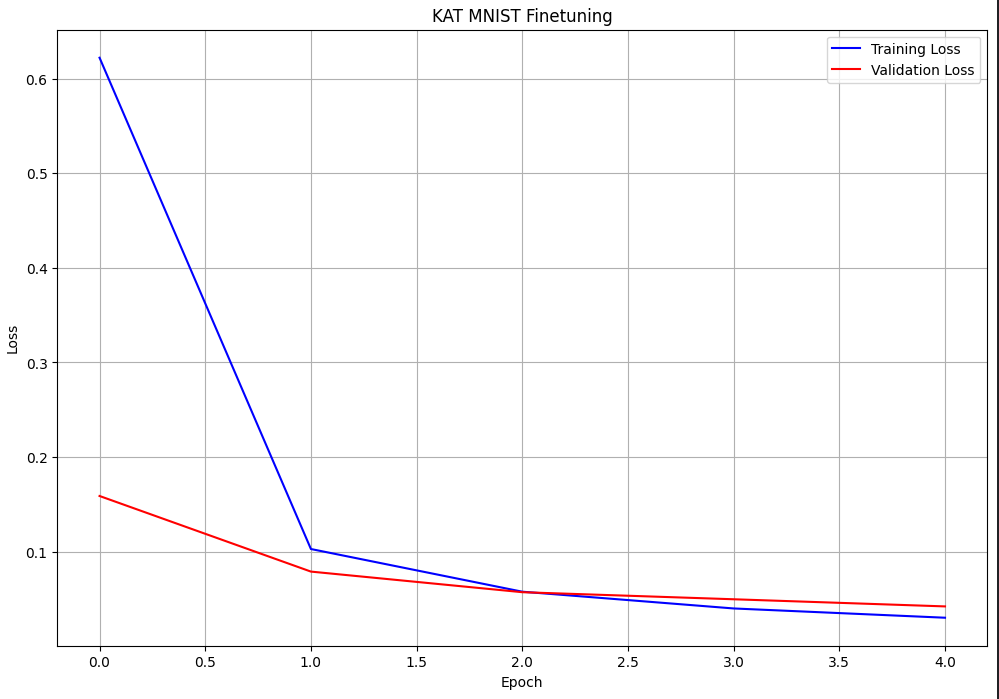
\includegraphics[width=0.65\linewidth]{mnist_train_val_loss.png}
    \caption{MNIST: Training (blue) vs.\ Validation (red) Loss.}
    \label{fig:mnist_loss}
\end{figure}

\begin{table}[H]
    \centering
    \scriptsize
    \begin{tabular}{lcccc}
        \toprule
        \textbf{Class}    & \textbf{Precision}          & \textbf{Recall} & \textbf{F1-score} & \textbf{Support} \\
        \midrule
        0                 & 0.99                        & 1.00            & 0.99              & 980              \\
        1                 & 0.99                        & 1.00            & 1.00              & 1135             \\
        2                 & 0.98                        & 1.00            & 0.99              & 1032             \\
        \ldots            & \ldots                      & \ldots          & \ldots            & \ldots           \\
        8                 & 0.99                        & 0.99            & 0.99              & 974              \\
        9                 & 0.99                        & 0.98            & 0.98              & 1009             \\
        \midrule
        \textbf{Accuracy} & \multicolumn{4}{c}{99.00\%}                                                          \\
        \bottomrule
    \end{tabular}
    \caption{MNIST Classification Report (partial).}
    \label{tab:mnist_report}
\end{table}

\subsection{FashionMNIST Finetuning Results}
FashionMNIST contains grayscale images of clothing items (10 classes) with an
original size of $28\times28$ \cite{fashionmnist}. The same preprocessing as
MNIST is applied.

Finetuning was also performed for 5 epochs using the AdamW optimizer in
conjunction with an early stopping mechanism, ultimately achieving a final test
accuracy of around 92.78\%.

\begin{figure}[H]
    \centering
    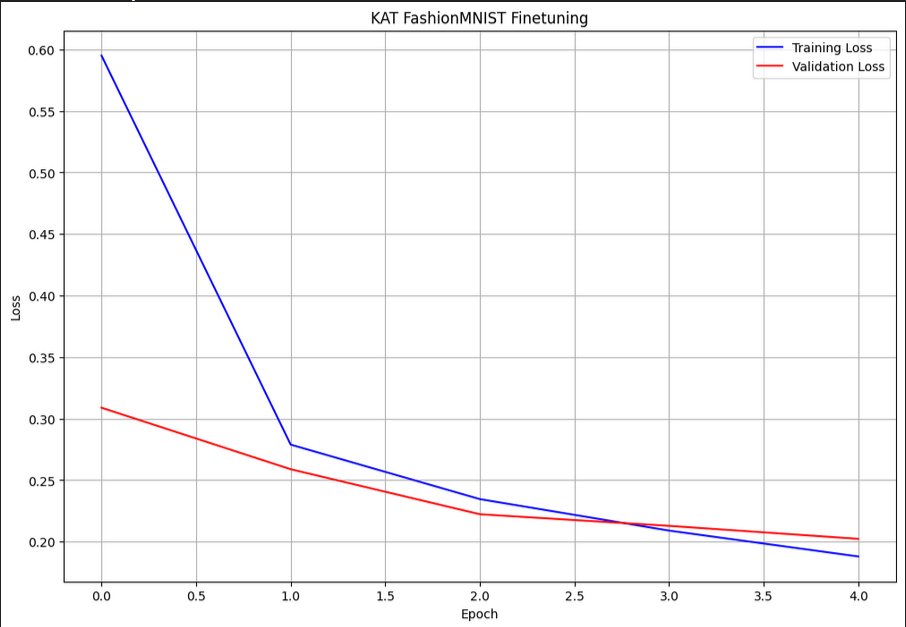
\includegraphics[width=0.55\linewidth]{fashionmnist_train_loss.png}
    \caption{FashionMNIST: Training vs.\ Validation Loss over 5 epochs.}
    \label{fig:fashionmnist_loss}
\end{figure}

\begin{table}[H]
    \centering
    \scriptsize
    \begin{tabular}{lcccc}
        \toprule
        \textbf{Class}    & \textbf{Precision}          & \textbf{Recall} & \textbf{F1-score} & \textbf{Support} \\
        \midrule
        0 (T-shirt/Top)   & 0.90                        & 0.85            & 0.87              & 1000             \\
        1 (Trouser)       & 0.99                        & 0.99            & 0.99              & 1000             \\
        2 (Pullover)      & 0.93                        & 0.87            & 0.90              & 1000             \\
        3 (Dress)         & 0.91                        & 0.92            & 0.92              & 1000             \\
        4 (Coat)          & 0.89                        & 0.93            & 0.91              & 1000             \\
        5 (Sandal)        & 0.99                        & 0.98            & 0.99              & 1000             \\
        6 (Shirt)         & 0.75                        & 0.82            & 0.79              & 1000             \\
        7 (Sneaker)       & 0.98                        & 0.95            & 0.96              & 1000             \\
        8 (Bag)           & 0.99                        & 0.99            & 0.99              & 1000             \\
        9 (Ankle Boot)    & 0.95                        & 0.98            & 0.97              & 1000             \\
        \midrule
        \textbf{Accuracy} & \multicolumn{4}{c}{93.01\%}                                                          \\
        \bottomrule
    \end{tabular}
    \caption{FashionMNIST Classification Report.}
    \label{tab:fashionmnist_report}
\end{table}

\subsection{CIFAR-10 Finetuning Results}
CIFAR-10 consists of 10 classes of color images (originally $32\times32$) which
are resized to $224\times224$ \cite{cifar}. Preprocessing involves
normalization with ImageNet statistics.

Similarly, for CIFAR-100, the model was finetuned over 5 epochs with early
stopping—where the best validation loss was recorded at epoch 5—and a final
test accuracy of approximately 95.70\% was obtained.

\begin{figure}[H]
    \centering
    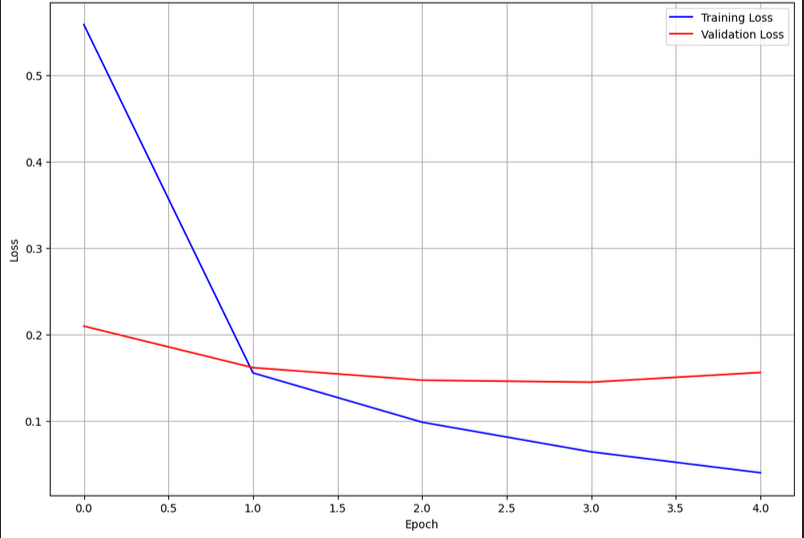
\includegraphics[width=0.55\linewidth]{cifar10_train_val_loss.png}
    \caption{CIFAR-10: Training vs.\ Validation Loss.}
    \label{fig:cifar10_loss}
\end{figure}

\begin{table}[H]
    \centering
    \scriptsize
    \begin{tabular}{lcccc}
        \toprule
        \textbf{Class}    & \textbf{Precision}          & \textbf{Recall} & \textbf{F1-score} & \textbf{Support} \\
        \midrule
        0 (Airplane)      & 0.98                        & 0.95            & 0.97              & 1000             \\
        1 (Automobile)    & 0.97                        & 0.98            & 0.97              & 1000             \\
        2 (Bird)          & 0.98                        & 0.95            & 0.97              & 1000             \\
        \ldots            & \ldots                      & \ldots          & \ldots            & \ldots           \\
        8 (Ship)          & 0.96                        & 0.99            & 0.98              & 1000             \\
        9 (Truck)         & 0.97                        & 0.96            & 0.97              & 1000             \\
        \midrule
        \textbf{Accuracy} & \multicolumn{4}{c}{95.70\%}                                                          \\
        \bottomrule
    \end{tabular}
    \caption{CIFAR-10 Classification Report (partial).}
    \label{tab:cifar10_report}
\end{table}

\subsection{CIFAR-100 Finetuning Results}
CIFAR-100 features 100 classes of color images (originally $32\times32$)
\cite{cifar} and is similarly preprocessed by resizing to $224\times224$ and
normalizing with ImageNet statistics.

Similarly, for CIFAR-100, the model was finetuned over 5 epochs with early
stopping—where the best validation loss was recorded at epoch 5—and a final
test accuracy of approximately 81.17\% was obtained.

\begin{figure}[H]
    \centering
    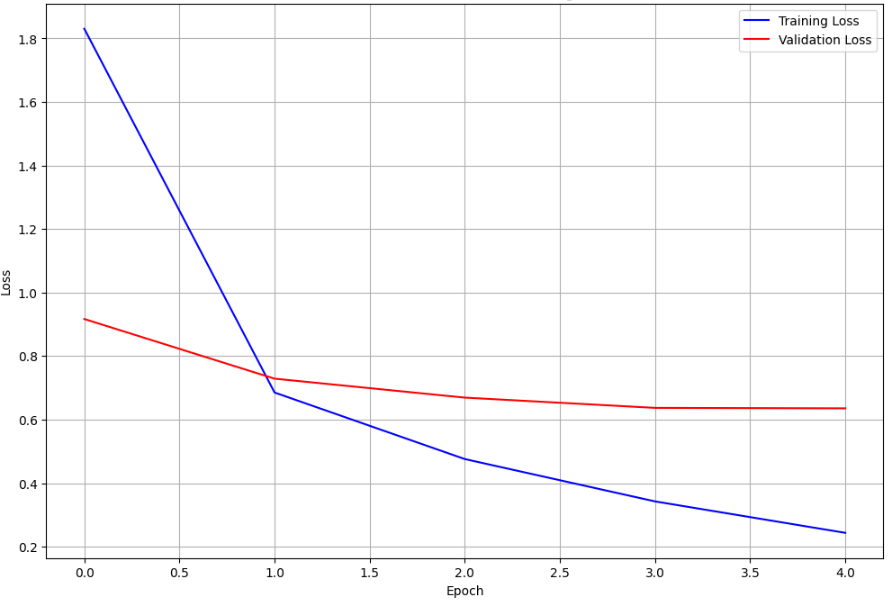
\includegraphics[width=0.55\linewidth]{cifar100_train_val_loss.png}
    \caption{CIFAR-100: Training vs.\ Validation Loss.}
    \label{fig:cifar100_loss}
\end{figure}

\begin{table}[H]
    \centering
    \scriptsize
    \begin{tabular}{lcccc}
        \toprule
        \textbf{Class}        & \textbf{Precision} & \textbf{Recall} & \textbf{F1-score} & \textbf{Support} \\
        \midrule
        Class 0               & 0.90               & 0.97            & 0.93              & 1000             \\
        Class 13              & 0.80               & 0.81            & 0.81              & 1000             \\
        Class 35              & 0.48               & 0.62            & 0.54              & 1000             \\
        \ldots                & \ldots             & \ldots          & \ldots            & \ldots           \\
        \midrule
        \textbf{Weighted Avg} & 0.82               & 0.81            & 0.81              & 10000            \\
        \bottomrule
    \end{tabular}
    \caption{CIFAR-100 Classification Report (excerpt).}
    \label{tab:cifar100_report}
\end{table}

\subsection{Summary of Finetuning Results}

Across all datasets, the finetuning procedure demonstrates that the pretrained
KAT model adapts efficiently to new tasks. Specifically, we achieved test
accuracies of approximately 99.33\% on MNIST, 93.01\% on FashionMNIST, 95.70\%
on CIFAR-10, and 81.17\% on CIFAR-100. These results highlight the versatility
of the KAT architecture, which effectively leverages large-scale pretrained
features and GPU parallelism to achieve strong performance on diverse image
recognition tasks within a short finetuning period. Moreover, the KAT model
effectively and efficiently retains the previously learned knowledge from
pretraining, adjusting quickly and properly to new information. Overall, our
results demonstrate the potential of KAT models for image recognition tasks and
the benefits of leveraging such pretrained models for efficient transfer
learning.

\subsection{Robustness Testing of Kolmogorov-Arnold Transformers (KAT)}

\subsubsection{Introduction}

Deep learning models are known to be sensitive to noisy and corrupted data,
which poses challenges in real-world scenarios where images are often degraded
by noise, occlusions, or other imperfections. Despite the rapid advancements in
neural network architectures, there is a limited understanding of how
Kolmogorov-Arnold Transformers (KAT) perform under such conditions. Thus we
decided to test how the the model finetuned on the MNIST dataset performs under
different types of noise and corruption.

\subsubsection{Methodology}

To evaluate the robustness of KAT models, three types of noise and corruption
were applied to the dataset: Gaussian noise, Salt \& Pepper noise, and
Occlusions. Gaussian noise was added to simulate random disturbances, while
Salt \& Pepper noise introduced pixel corruption. Occlusions were implemented
by randomly blocking sections of images. The objective was to assess how each
type of perturbation affects the model's performance. The models were
fine-tuned using cross-entropy loss with the AdamW optimizer and evaluated
using accuracy metrics and confusion matrices.

\subsubsection{Results}

The experiments revealed that KAT models exhibit varying levels of robustness
depending on the type and severity of noise. When tested with Gaussian noise,
the accuracy dropped from 80\% to 77.12\%, indicating a moderate decline in
performance. In the case of Salt \& Pepper noise, the accuracy further
decreased to 69.7\%, suggesting a higher sensitivity to pixel corruption.
Occlusions had the most significant impact, reducing accuracy to 63.92\%. These
results demonstrate that performance degradation is correlated with noise
severity.

\subsubsection{Analysis \& Discussion}

The analysis shows that KAT models maintain relatively high accuracy under
moderate noise conditions but are particularly sensitive to severe occlusions.
Compared to traditional Convolutional Neural Networks (CNNs), KAT models
demonstrate robust performance, although they are outperformed by models
utilizing advanced augmentation techniques. The findings highlight the need for
enhanced augmentation strategies and hybrid model architectures to improve
robustness against heavy corruption.

\subsubsection{Conclusion}

We conclude that Kolmogorov-Arnold Transformers (KAT) are generally robust to
moderate noise but face challenges under severe image corruption. Future work
will focus on investigating robustness against adversarial attacks and
exploring real-world noise scenarios. Additionally, further research on hybrid
architectures and improved data augmentation techniques could enhance model
performance in noisy environments.

\section{Kanvolutional Layer}

As explored in \cite{CNN-KAN}, the combination of convolutions with KANs
introduces computational limitations due to the high number of parameters and
the inherently non-parallelizable nature of the approach. Inspired by [x:
        KAT-Transformer], we propose the use of rational functions, which enable highly
parallel implementations while significantly reducing the number of parameters
compared to convolutions with B-splines as activation functions.This work paves
the way for novel architectures with greater expressive power and improved
convergence properties. We introduce the Kanvolutional layer, a
convolution-like layer integrated with nonlinear, learnable functions instead
of scalar weights. The learnable function is defined as follows:

\begin{equation*}
    \phi(x) := \frac{a_0 + a_1x + a_2x^2 + \dots + a_nx^p}{1 + |b_1x + b_2x^2 + \dots + b_mx^q|}
\end{equation*}

A Kanvolution operation is analogous to a conventional convolution operation;
however, instead of performing element-wise multiplications between the image
and kernel elements, it involves the composition of the kernel's learnable
function with the elements of the image.

More concretly a conventional kernel $\mathbf{K} \in R^{2 \times 2}$ consists
of four scalar values:

\begin{equation*}
    \mathbf{K} =    \begin{bmatrix}
        w_{11} & w_{12} \\
        w_{21} & w_{22}
    \end{bmatrix}
\end{equation*}

while a kanvolutional kernel $\mathbf{K_\phi} \in R^{2 \times 2}$ consists of
four learnable functions:

\begin{equation*}
    \mathbf{K_\phi}= \begin{bmatrix}
        w_{11}\phi_{11}(\cdot) & w_{12}\phi_{12}(\cdot) \\
        w_{21}\phi_{21}(\cdot) & w_{22}\phi_{22}(\cdot)
    \end{bmatrix}
\end{equation*}

Finally, the Kanvolution operation is defined as follows:
\begin{multline*}
    \mathbf{K}_{\phi} * \mathbf{I} = \\ \\
    \left[
        \begin{array}{cc}
            \scriptstyle w_{11}K_{\phi_{11}}(I_{11}) + w_{12}K_{\phi_{12}}(I_{12}) \\
            + w_{21}K_{\phi_{21}}(I_{21})                                          \\
            + w_{22}K_{\phi_{22}}(I_{22}),                               &
            \scriptstyle w_{11}K_{\phi_{11}}(I_{12})                               \\
            + w_{12}K_{\phi_{12}}(I_{13})                                          \\
            + w_{21}K_{\phi_{21}}(I_{22}) + w_{22}K_{\phi_{22}}(I_{23})            \\
            \scriptstyle w_{11}K_{\phi_{11}}(I_{21})                               \\
            + w_{12}K_{\phi_{12}}(I_{22})                                          \\
            + w_{21}K_{\phi_{21}}(I_{31}) + w_{22}K_{\phi_{22}}(I_{32}), &
            \scriptstyle w_{11}K_{\phi_{11}}(I_{22})                               \\
            + w_{12}K_{\phi_{12}}(I_{23})
            \\ + w_{21}K_{\phi_{21}}(I_{32}) + w_{22}K_{\phi_{22}}(I_{33})
        \end{array}
        \right]
\end{multline*}

where $\mathbf{I} \in \mathbb{R}^{3 \times 3}$ represents a single-channel
image, and $\textbf{K}_{\phi} \in \mathbb{R}^{2 \times 2}$ denotes a
Kanvolutional kernel.

A conventional convolutional 2D layer has $$ c_{out} \times c_{in} \times k_h
    \times k_w $$ parameters, while a Kanvolutional 2D layer has $$ c_{out} \times
    c_{in} \times (o_p+1) \times o_q \ \times k_h \times k_w $$ parameters. Here,
\( o_p \) denotes the order of the polynomial in the numerator, while \( o_q \)
represents the order of the polynomial in the denominator.

\subsection{Weight Initialization}

The choice of an appropriate initialization scheme plays a crucial role in
neural network training, significantly impacting numerical stability and
convergence. The initial scheme involved drawing weights from a uniform
distribution

$$
    U\left(-k^{-1/p}, k^{-1/p}\right)
$$

for the numerator of \( \phi \), while for the denominator, the weights were
sampled from

$$
    U\left(-k^{-1/(q+1)}, k^{-1/(q+1)}\right)
$$

to appropriately scale the higher-order polynomial terms. However, this
initialization did not yield the desired results. Consequently, we adopted
PyTorch's approach, initializing the weights using the uniform distribution

$$
    U\left(-\sqrt{k}, \sqrt{k}\right)
$$

where \( k \) represents the size of the kernel.

\subsection{Training}
For training and evaluating our Kanvolutional layer, we used the MNIST and
Fashion-MNIST datasets. For comparison purposes, we constructed a neural
network with two Kanvolutional layers and one linear layer, maintaining the
same architectural structure and ensuring that each Kanvolutional layer
produced the same number of outputs as in \cite{CNN-KAN}. Notably, we did not
use any activation functions (e.g., ReLU, GELU, etc.) in the network.

Initially, we experimented with the polynomial orders \( p \) and \( q \). We
observed that for high-order polynomials, the neural network performed
similarly to configurations with lower-order polynomials. For the loss
function, we used cross-entropy, and for optimization, we employed AdamW.

We initially set the learning rate to \(10^{-4}\), but early in training, we
noticed that the training loss remained stagnant. To address this issue, we
implemented a step-based linear scheduler, starting with a learning rate of
\(10^{-2}\), which was reduced by half every five epochs. Additionally, during
training, we employed early stopping to prevent redundant epochs and avoid
overfitting.

We did not apply data augmentation, as we believed it could introduce
additional variability and lead to overly optimistic results regarding the
effectiveness of the Kanvolutional layer.

\subsection{Results}

The results of the experiments are presented in Table \ref{ressfashion}. Our
approach achieves an accuracy exceeding 90\%, outperforming all tested models.
As seen in Table \ref{ressfashion}, a smaller variant of our approach, which
uses only half the number of parameters, also performs well, still surpassing
other methods. In the table, \( o_{c} \) (in parentheses) indicates the number
of output channels for each Kanvolutional or convolutional layer, while
\textit{gs} represents the grid size for the internal B-spline. The runtime per
epoch is not directly comparable, as the implementation of Kanvolutional layers
is not optimized for CUDA, unlike standard convolution operations.

\begin{table}[h]
    \centering
    \begin{tabular}{l|c|c}
        \hline
        \textbf{Model}                                                & \textbf{Accuracy} & \textbf{\#Params} \\
        \hline
        \textbf{KonVNet} (Ours: \(o_c = 10\), \(o_c = 20\))           & \textbf{90.32\%}  & 18.3K             \\
        \textbf{KonVNet} (Ours medium: \(o_c = 5\), \(o_c = 10\))     & 89.94\%           & 6K                \\
        CNN (Medium+: \(o_c = 5\), \(o_c = 10\))                      & 89.56\%           & 6.93K             \\
        CNN (Big: \(o_c = 5\), \(o_c = 10\) + 2 FC layers)            & 89.44\%           & 26.62K            \\
        CNN (Medium: \(o_c = 5\), \(o_c = 10\))                       & 88.34\%           & 3.02K             \\
        CNN (Small: \(o_c = 5\), \(o_c = 5\))                         & 87.10\%           & 1.54K             \\
        KANC MLP (Big: \(o_c = 5\), \(o_c = 10\) + 2 FC, \(gs = 10\)) & 89.15\%           & 33.54K            \\
        KANC MLP (Big: \(o_c = 5\), \(o_c = 10\) + 2 FC, \(gs = 20\)) & 89.11\%           & 38.48K            \\
        KANC MLP (Medium: \(o_c = 5\), \(o_c = 10\)) (\(gs = 10\))    & 88.99\%           & 9.94K             \\
        KANC MLP (Medium: \(o_c = 5\), \(o_c = 10\)) (\(gs = 20\))    & 88.90\%           & 14.89K            \\
        KANC MLP (Small: \(o_c = 5\), \(o_c = 5\)) (\(gs = 10\))      & 87.43\%           & 5.31K             \\
        KANC MLP (Small: \(o_c = 5\), \(o_c = 5\)) (\(gs = 20\))      & 88.15\%           & 8.01K             \\
        KKAN (Medium: \(o_c = 5\), \(o_c = 10\)) (\(gs = 10\))        & 87.91\%           & 44.93K            \\
        KKAN (Medium: \(o_c = 5\), \(o_c = 10\)) (\(gs = 20\))        & 88.56\%           & 74.88K            \\
        KKAN (Small: \(o_c = 5\), \(o_c = 5\)) (\(gs = 10\))          & 88.01\%           & 22.80K            \\
        KKAN (Small: \(o_c = 5\), \(o_c = 5\)) (\(gs = 20\))          & 87.94\%           & 38.00K            \\
        \hline
    \end{tabular}
    \caption{Experiments on Fashion MNIST}
    \label{ressfashion}
\end{table}

\subsection{Future work}

For future work, a primary focus should be the CUDA implementation to assess
the computational speed of the neural network and compare its efficiency with
conventional convolutional layers.In our repository, we provide
\textit{u-kanvolutional-net}, a neural network built using Kanvolutional
layers. Researchers can build upon this framework, extending these ideas to
explore new applications and conduct further evaluations. Another exciting
direction is the choice of activation functions. In this work, we used a
rational function; however, exploring alternative activation functions could
potentially reduce the number of parameters even further. Investigating the
trade-off between parameter reduction and network performance would be a
valuable avenue for future research.

\section{U-KAN Architecture: A Hybrid Approach}

\IEEEPARstart{M}{edical} image segmentation is a critical task in computer-aided diagnosis, surgical planning, and disease monitoring. Traditional deep learning architectures, such as U-Net, have become the standard for medical image analysis. However, despite their success, these models exhibit key limitations :

\setlength{\parskip}{0pt}
\begin{enumerate}[label=\arabic*.] % The 'label' option specifies the format
    \item \textbf{Linear Modeling Limitations:} U-Net and its derivatives (U-Net++, V-Net, Y-Net) rely on convolutional and transformer-based architectures, which struggle to model complex nonlinear patterns in medical images.
    \item \textbf{Lack of Interpretability:}Most deep learning models function as black boxes, making them less trustworthy for clinical applications.
    \item \textbf{Computational Overhead:}Transformer-based architectures provide global feature learning but are computationally expensive and prone to overfitting, especially on limited medical datasets.
\end{enumerate}

We will explore the ideas presented in \cite{arxiv2406} by implementing U-KAN,
a novel U-Net variant that incorporates Kolmogorov-Arnold Networks (KANs) to
enhance the model’s capability in capturing nonlinear dependencies while also
improving computational efficiency and interpretability.

\subsection{Limitations of Conventional U-Net Architectures}
Despite its widespread adoption, U-Net and its derivatives (U-Net++, V-Net,
Swin-UNet) suffer from several deficiencies:

\setlength{\parskip}{0pt}
\begin{enumerate}[label=\arabic*.] % The 'label' option specifies the format
    \item \textbf{Convolutional Neural Network:} CNN-based models often struggle to generalize effectively across diverse anatomical structures due to their inherently limited receptive fields. The receptive field in a CNN refers to the region of the input image that a neuron can "see" at a given layer. Although deeper layers can capture more abstract and global features, the model primarily relies on local spatial dependencies. This localized processing can be insufficient when analyzing complex anatomical variations, where global context and long-range dependencies play a crucial role.
    \item \textbf{Transformer-based models} like TransUNet enhance global feature learning by capturing long-range dependencies but suffer from high memory consumption due to self-attention's quadratic complexity. They are also prone to overfitting, particularly in medical imaging with limited training data.
    \item \textbf{MLP-based models}  (e.g., U-NeXt, Rolling-UNet) attempt to bridge this gap but still rely on linear transformations, restricting their ability to model intricate spatial dependencies.
\end{enumerate}

By replacing traditional MLP layers with KAN layers, U-KAN provides an
efficient backbone for segmentation and generative modeling, enhancing
representation learning while maintaining computational efficiency.

\subsection{U-KAN Model Architecture}
U-KAN employs a two-stage encoder-decoder pipeline, incorporating KAN layers
during feature extraction to enhance representation learning and improve
segmentation and generative modeling performance.

\setlength{\parskip}{0pt}
\begin{enumerate}[label=\arabic*.] % The 'label' option specifies the format
    \item \textbf{Encoder Phase:} The encoder starts with convolutional layers to capture low-level spatial features. These feature maps are then tokenized into patch embeddings, enabling KAN-based transformations for improved feature abstraction and contextual learning.
    \item \textbf{Tokenized KAN Layers:} Feature representations are converted into tokenized feature vectors for structured processing. Instead of MLPs, KAN layers are applied, enhancing nonlinear modeling through learnable activation functions, leading to more flexible and adaptive feature learning.
    \item \textbf{Decoder Phase:}  Skip connections preserve spatial information, while feature maps are progressively upsampled to reconstruct high-resolution outputs, refining segmentation masks with enhanced detail.
\end{enumerate}

\begin{figure}[h!] % 'h' means "here" (try to place it at this location)
    \centering % Centers the image
    \includegraphics[width=0.4\textwidth]{data_kan/ukan_architecture.png} % Adjust width
    \caption{Overview of the U-KAN pipeline: Following feature extraction through multiple convolutional blocks in the Convolution Phase, the intermediate feature maps undergo tokenization and are processed by a series of stacked Tok-KAN blocks in the Tokenized KAN Phase. When used in Diffusion U-KAN, time embedding is incorporated exclusively within the KAN blocks.} % Caption for the image
    \label{fig:example} % Reference label
\end{figure}

\subsection{Experimental Evaluation}

\subsubsection{Dataset}
The \textbf{BKAI-IGH NeoPolyp} dataset is designed for \textit{polyp
    segmentation and neoplasm classification} in colonoscopy images. It is widely
used in medical imaging research, particularly for gastrointestinal (GI)
endoscopy.

The dataset consists of \textbf{1,200 images}, divided into:
\begin{itemize}
    \item \textbf{1,000 training images}
    \item \textbf{200 test images}
\end{itemize}
These images come from two different imaging modalities:
\begin{itemize}
    \item White Light Imaging (WLI) - 1,000 images
    \item Flexible Spectral Imaging Color Enhancement (FICE) - 200 images
\end{itemize}
Each image has manually annotated \textit{segmentation masks} to define polyp regions.

\subsubsection{Tasks and Challenges}
\begin{itemize}

    \item{\textbf{Polyp Segmentation}:} The goal is to detect and delineate \textbf{polyp regions} from colonoscopy images, which helps in \textit{computer-aided diagnosis (CADx)}. Deep learning models like \textbf{U-Net} and \textbf{DeepLabV3} are commonly used.

    \item{\textbf{Neoplasm Characterization}:} The dataset supports classification tasks to distinguish between \textbf{neoplastic} (pre-cancerous/cancerous) and \textbf{non-neoplastic} (benign) polyps. Models like ResNet and U-Net are often applied.

\end{itemize}

\textbf{Challenges}
\begin{itemize}
    \item High variability in polyp size, shape, and texture.
    \item Class imbalance in neoplastic vs. non-neoplastic cases.
    \item Presence of imaging artifacts such as motion blur and fluids.
    \item Limited dataset size for deep learning applications.
\end{itemize}

\subsubsection{Performance Metrics}

Segmentation accuracy is commonly evaluated using the \textbf{Intersection over
    Union (IoU)} and the \textbf{Dice Coefficient}, both of which measure the
overlap between predicted and ground truth segmentation masks.

\textbf{Intersection over Union (IoU):}
The Intersection over Union (IoU), also known as the Jaccard index, quantifies the similarity between the predicted segmentation mask \( A \) and the ground truth mask \( B \). It is defined as:

\begin{equation}
    IoU = \frac{|A \cap B|}{|A \cup B|}
\end{equation}

IoU ranges from 0 to 1, where a higher IoU indicates a better segmentation
performance.

\textbf{Dice Coefficient (DSC):}
The Dice coefficient, also called the Dice Similarity Coefficient (DSC), measures the harmonic mean of precision and recall, defined as:

\begin{equation}
    Dice = \frac{2|A \cap B|}{|A| + |B|}
\end{equation}

The Dice coefficient ranges from 0 to 1, where a value of 1 indicates a perfect
segmentation match, and 0 indicates no overlap. This metric is particularly
useful in medical image segmentation due to its sensitivity to small
structures.

Both metrics are widely used in segmentation tasks, with the Dice coefficient
being more sensitive to smaller regions, while IoU provides a stricter
evaluation by penalizing false positives and false negatives.

\subsubsection{Experimental Evaluation}
\vspace{1em}
We conducted a comprehensive evaluation of segmentation performance by testing two deep learning architectures, \textbf{U-Net} and \textbf{U-KAN}, on the given dataset. The primary objective of this evaluation was to assess the effectiveness of these models in accurately segmenting anatomical structures while considering key performance metrics.

To ensure a rigorous comparison, both models were trained under identical
conditions, utilizing the same dataset splits for training, validation, and
testing. The evaluation metrics include the \textbf{Intersection over Union
    (IoU)} and the \textbf{Dice Similarity Coefficient (DSC)}, which are widely
used to quantify the degree of overlap between predicted and ground truth
segmentation masks.

The results of our experiments, detailing the segmentation accuracy of U-Net
and U-KAN, are presented in the following sections. These findings provide
insights into the comparative advantages and limitations of each architecture,
particularly in handling complex anatomical structures and varying spatial
features.

\begin{figure}[h!]
    \centering
    % IoU Image
    \includegraphics[width=0.4\textwidth]{data_kan/ukan_iou.png}
    \caption{Intersection over Union comparison between U-Net and U-KAN.}
    \label{fig:iou}

    \vspace{10pt} % Adds space between images

    % Dice Image
    \includegraphics[width=0.4\textwidth]{data_kan/ukan_dice.png}
    \caption{Dice Similarity Coefficient comparison between U-Net and U-KAN.}
    \label{fig:dice}
\end{figure}

\begin{table}[h!]
    \centering
    \begin{tabular}{|c|c|c|c|}
        \hline
        \textbf{Model} & \textbf{Epoch} & \textbf{IoU} & \textbf{Dice} \\
        \hline
        U-KAN          & 86             & 0.6910       & 0.8091        \\
        U-Net          & 72             & 0.6916       & 0.8107        \\
        \hline
    \end{tabular}
    \caption{Segmentation performance comparison of U-Net and U-KAN.}
    \label{tab:results}
\end{table}

\subsubsection{Computational Efficiency}

Beyond segmentation accuracy, we evaluated the computational efficiency of both
models. Notably, \textbf{U-KAN requires approximately 93\% fewer FLOPs than
    U-Net}, representing a substantial reduction in computational complexity. This
efficiency gain is attributed to the replacement of conventional MLP layers
with KAN layers, which enhance feature learning while minimizing redundant
operations.

The drastic decrease in FLOP count makes U-KAN highly suitable for deployment
in resource-constrained environments, such as real-time medical imaging
applications. This balance between \textbf{high segmentation accuracy and
    significantly reduced computational overhead} underscores the potential of
U-KAN as an optimized alternative to traditional CNN-based architectures.

\subsection{Conclusion and Future Work}

We conducted a comparative analysis between \textbf{U-Net} and \textbf{U-KAN}
for medical image segmentation, evaluating their performance in terms of
accuracy, computational efficiency, and interpretability. Our findings
demonstrate that while both models achieve comparable segmentation accuracy,
\textbf{U-KAN significantly reduces computational costs}, making it a promising
alternative for real-time and resource-constrained medical applications.

\subsubsection{Key Findings}

\begin{itemize}
    \item \textbf{Segmentation Performance}: U-Net and U-KAN performed similarly in segmentation accuracy, with U-Net achieving an \textbf{IoU of 0.6916} and a \textbf{Dice coefficient of 0.8107}, while U-KAN achieved an \textbf{IoU of 0.6910} and a \textbf{Dice coefficient of 0.8091}.

    \item \textbf{Computational Efficiency}: A major advantage of U-KAN is its significantly \textbf{lower computational cost}, requiring approximately \textbf{93\% fewer FLOPs} than U-Net. This efficiency is due to replacing traditional MLP layers with \textbf{Kolmogorov-Arnold Networks (KANs)}, which model nonlinear dependencies effectively with fewer parameters.

    \item \textbf{Interpretability and Scalability}: Unlike traditional CNN-based architectures, U-KAN offers \textbf{greater model interpretability}, as KANs provide structured feature decomposition. The lightweight nature of U-KAN makes it particularly \textbf{scalable to larger medical datasets} and deployable in \textbf{real-time clinical environments}.
\end{itemize}

\subsubsection{Future Research Directions}

To further improve the applicability of U-KAN, future research should focus on
the following areas:

\begin{enumerate}
    \item \textbf{Enhancing Feature Representation}
          \begin{itemize}
              \item Incorporating \textbf{multi-scale learning mechanisms} to capture both global
                    and local spatial dependencies.
              \item Investigating hybrid architectures that \textbf{combine KANs with CNNs or
                        transformers} to improve hierarchical feature extraction.
          \end{itemize}

    \item \textbf{Expanding to New Medical Domains}
          \begin{itemize}
              \item Extending U-KAN to \textbf{3D segmentation} for volumetric medical images
                    (e.g., \textbf{MRI, CT scans}) to improve applications in \textbf{organ
                        segmentation and tumor detection}.
              \item Investigating its performance in \textbf{genomic and multimodal AI},
                    integrating medical images with \textbf{clinical text, pathology reports, and
                        genetic data}.
          \end{itemize}

    \item \textbf{Optimizing for Real-Time Clinical Deployment}
          \begin{itemize}
              \item Developing \textbf{hardware-aware implementations} to leverage GPUs and
                    \textbf{low-power AI accelerators} for faster inference on embedded devices.
              \item Optimizing U-KAN for \textbf{mobile health applications and edge computing},
                    enabling AI-driven segmentation for \textbf{remote diagnostics} in
                    resource-constrained settings.
          \end{itemize}
\end{enumerate}

\subsubsection{Final Remarks}
The findings highlight the importance of exploring \textbf{mathematically
    inspired neural network architectures} as viable alternatives to conventional
deep learning models. Future advancements in \textbf{lightweight segmentation
    networks} could significantly improve the adoption of AI in \textbf{clinical
    workflows}, ultimately enhancing accessibility to high-quality, automated
medical image analysis and contributing to better patient outcomes.

\bibliography{bib}
\bibliographystyle{plainnat}

% Force a new page after references
\clearpage
\onecolumn
\appendix

\section{Appendix}

\noindent
The scripts for experiments and analysis are available in the following GitHub repository: \url{https://github.com/panos-span/patrec_kan}.


\subsection{Differential Equations Hyperparameter Tuning}

% Table 1: Final Results Summary
\begin{table*}[ht]
    \centering
    \resizebox{\textwidth}{!}{%
        \begin{tabular}{|c|c|c|c|c|c|c|c|c|}
            \hline
            \textbf{Alpha} & \textbf{Learning Rate} & \textbf{Grid} & \textbf{Hidden Layers}      & \textbf{Steps} & \textbf{Final PDE Loss} & \textbf{Final BC Loss} & \textbf{Final L2 Loss} \\ \hline
            0.01           & 0.1                    & 20            & $\{[2,0],\,[2,0],\,[1,0]\}$ & 50             & 0.098931484             & $4.11614\times10^{-5}$ & $7.74674\times10^{-5}$ \\ \hline
            0.01           & 0.1                    & 20            & $\{[2,0],\,[2,0],\,[1,0]\}$ & 100            & 0.09734199              & $3.01013\times10^{-5}$ & $6.79842\times10^{-5}$ \\ \hline
            0.01           & 0.1                    & 20            & $\{[2,0],\,[4,0],\,[1,0]\}$ & 50             & 0.01661489              & $7.79619\times10^{-5}$ & $1.91280\times10^{-5}$ \\ \hline
            0.01           & 0.1                    & 20            & $\{[2,0],\,[4,0],\,[1,0]\}$ & 100            & 0.00936218              & $2.22028\times10^{-5}$ & $7.07273\times10^{-6}$ \\ \hline
            0.01           & 1.0                    & 20            & $\{[2,0],\,[2,0],\,[1,0]\}$ & 50             & 0.099617355             & $3.88579\times10^{-5}$ & $8.13428\times10^{-5}$ \\ \hline
            0.01           & 1.0                    & 20            & $\{[2,0],\,[2,0],\,[1,0]\}$ & 100            & 0.097212814             & $3.10407\times10^{-5}$ & $6.88948\times10^{-5}$ \\ \hline
            0.01           & 1.0                    & 20            & $\{[2,0],\,[4,0],\,[1,0]\}$ & 50             & 0.012592219             & $3.58469\times10^{-5}$ & $5.91649\times10^{-6}$ \\ \hline
            0.01           & 1.0                    & 20            & $\{[2,0],\,[4,0],\,[1,0]\}$ & 100            & 0.01139089              & $2.06362\times10^{-5}$ & $1.15428\times10^{-5}$ \\ \hline
            0.10           & 0.1                    & 20            & $\{[2,0],\,[2,0],\,[1,0]\}$ & 50             & 0.11535645              & 0.0261043              & 0.00793130             \\ \hline
            0.10           & 0.1                    & 20            & $\{[2,0],\,[2,0],\,[1,0]\}$ & 100            & 0.074458875             & 0.00106522             & 0.000463707            \\ \hline
            0.10           & 0.1                    & 20            & $\{[2,0],\,[4,0],\,[1,0]\}$ & 50             & 0.01671233              & 0.00207706             & 0.000513860            \\ \hline
            0.10           & 0.1                    & 20            & $\{[2,0],\,[4,0],\,[1,0]\}$ & 100            & 0.00885708              & 0.000421492            & 0.000201921            \\ \hline
            0.10           & 1.0                    & 20            & $\{[2,0],\,[2,0],\,[1,0]\}$ & 50             & 0.13935494              & 0.01612986             & 0.00514839             \\ \hline
            0.10           & 1.0                    & 20            & $\{[2,0],\,[2,0],\,[1,0]\}$ & 100            & 0.09209691              & 0.00566467             & 0.00167702             \\ \hline
            0.10           & 1.0                    & 20            & $\{[2,0],\,[4,0],\,[1,0]\}$ & 50             & 0.01556281              & 0.00228453             & 0.000498032            \\ \hline
            0.10           & 1.0                    & 20            & $\{[2,0],\,[4,0],\,[1,0]\}$ & 100            & 0.01576780              & 0.00171363             & 0.000378690            \\ \hline
        \end{tabular}%
    }
    \caption{Final Results Summary for Example 1}
    \label{tab:final_results}
\end{table*}

% Table 2: Hyperparameter Tuning Results for the MLP Model for Example 1
\begin{table*}[ht]
    \centering
    \resizebox{\textwidth}{!}{%
        \begin{tabular}{|c|c|c|c|c|c|c|c|c|c|}
            \hline
            \textbf{Learning Rate} & \textbf{Hidden Dim} & \textbf{Batch Size} & \textbf{Max Norm} & \textbf{PDE Loss} & \textbf{BC Loss} & \textbf{Total Loss} & \textbf{Training Time (s)} & \# \textbf{Parameters} & \textbf{Alpha} \\ \hline
            0.0010                 & 50                  & 256                 & 0.5               & 0.0109            & 0.000012         & 0.000120            & 78.946                     & 2751                   & 0.01           \\ \hline
            0.0010                 & 50                  & 256                 & 0.5               & 0.0066            & 0.000122         & 0.000780            & 81.301                     & 2751                   & 0.1            \\ \hline
            0.0010                 & 50                  & 256                 & 1.0               & 0.0108            & 0.000004         & 0.000112            & 76.889                     & 2751                   & 0.01           \\ \hline
            0.0010                 & 50                  & 256                 & 1.0               & 0.0056            & 0.000064         & 0.000629            & 78.707                     & 2751                   & 0.1            \\ \hline
            0.0010                 & 50                  & 512                 & 0.5               & 0.0141            & 0.000052         & 0.000193            & 105.880                    & 2751                   & 0.01           \\ \hline
            0.0010                 & 50                  & 512                 & 0.5               & 0.0031            & 0.000023         & 0.000331            & 101.380                    & 2751                   & 0.1            \\ \hline
            0.0010                 & 50                  & 512                 & 1.0               & 0.0032            & 0.000009         & 0.000041            & 101.820                    & 2751                   & 0.01           \\ \hline
            0.0010                 & 50                  & 512                 & 1.0               & 0.0046            & 0.000094         & 0.000557            & 121.250                    & 2751                   & 0.1            \\ \hline
            0.0010                 & 100                 & 256                 & 0.5               & 0.0108            & 0.000016         & 0.000124            & 114.180                    & 10501                  & 0.01           \\ \hline
            0.0010                 & 100                 & 256                 & 0.5               & 0.0012            & 0.000006         & 0.000122            & 111.210                    & 10501                  & 0.1            \\ \hline
            0.0010                 & 100                 & 256                 & 1.0               & 0.0041            & 0.000011         & 0.000052            & 128.340                    & 10501                  & 0.01           \\ \hline
            0.0010                 & 100                 & 256                 & 1.0               & 0.0040            & 0.000066         & 0.000469            & 127.300                    & 10501                  & 0.1            \\ \hline
            0.0010                 & 100                 & 512                 & 0.5               & 0.0046            & 0.000005         & 0.000051            & 208.080                    & 10501                  & 0.01           \\ \hline
            0.0010                 & 100                 & 512                 & 0.5               & 0.0005            & 0.000020         & 0.000066            & 179.470                    & 10501                  & 0.1            \\ \hline
            0.0010                 & 100                 & 512                 & 1.0               & 0.0064            & 0.000009         & 0.000073            & 176.250                    & 10501                  & 0.01           \\ \hline
            0.0010                 & 100                 & 512                 & 1.0               & 0.0028            & 0.000036         & 0.000312            & 176.600                    & 10501                  & 0.1            \\ \hline
            0.0001                 & 50                  & 256                 & 0.5               & 0.2493            & 0.000322         & 0.002815            & 75.976                     & 2751                   & 0.01           \\ \hline
            0.0001                 & 50                  & 256                 & 0.5               & 0.0646            & 0.000668         & 0.007127            & 73.934                     & 2751                   & 0.1            \\ \hline
            \bottomrule
        \end{tabular}%
    }
    \caption{Hyperparameter tuning results for the MLP model for Example~1.}
    \label{tab:mlp_hyperparam_tuning}
\end{table*}

\end{document}

